%%%%Internal Cryogenics%%%%
\label{sec:fdsp-tc-internal-cryo}

The internal cryogenics is comprised of three sets of pipe distribution networks and two sets of sprayers. All pipes enter the cryostat from the top, some go all the way down to the floor, others remain in the ceiling. On the floor there are:
\begin{itemize}
\setlength\itemsep{1mm}
\setlength{\parsep}{1mm}
\setlength{\itemsep}{-5mm}
\item \textbf{Gaseous argon (GAr) distribution}. A set of pipes flowing GAr. They are used only at the beginning to remove the air that fills the cryostat. They have either a longitudinal slit or calibrated holes to distribute the GAr uniformly along the length of the cryostat. Computational Fluid Dynamic (CFD) simulations show that air will be removed from the system, as long as GAr is flowing in at the right speed, calculated and experimentally verified as \SI{1.2}{m/hr}.

\item \textbf{\dword{lar} distribution}. Two sets of pipes flowing \dword{lar}. They are used to fill the cryostat and during steady--state operations to return the \dword{lar} from the purification system. The pipes have calibrated holes to return the \dword{lar} uniformly throughout the length of the cryostat. This is very important for the uniformity of the purity. Four pumps circulate the \dword{lar}. Initially all of them are in operation to achieve purity, but once the target purity has been achieved, only one or two remain in service. Two sets of pipes are needed to adequately distribute the \dword{lar} over this broad range of flow rates.
\end{itemize}

On the ceiling there are:

\begin{itemize}
\setlength\itemsep{1mm}
\setlength{\parsep}{1mm}
\setlength{\itemsep}{-5mm}
\item \textbf{Cool--down sprayers}. Two sets of cool--down sprayers are distributed along the long sides of each cryostat. One set distributes \dword{lar} using liquid sprayers that generate a conical profile of small droplets of liquid. Another set distributes GAr to move the \dword{lar} droplets inside and cool down the detector and cryostat uniformly. These sprayers are being tested in \dword{pddp}. They are a variation of those implemented in \dword{pdsp}.
\end{itemize}

The current layout of the internal cryogenics is shown on Figure~\ref{fig:internal-cryo-3D}. The current drawing of the internal cryogenics is presented in Figure~\ref{fig:internal-cryo-drawing}. The GAr pipes are depicted in red, the \dword{lar} pipes in blue.

\begin{dunefigure}[Cryogenic piping inside the cryostat ]{fig:internal-cryo-3D}
  {Layout of the internal cryogenics.}
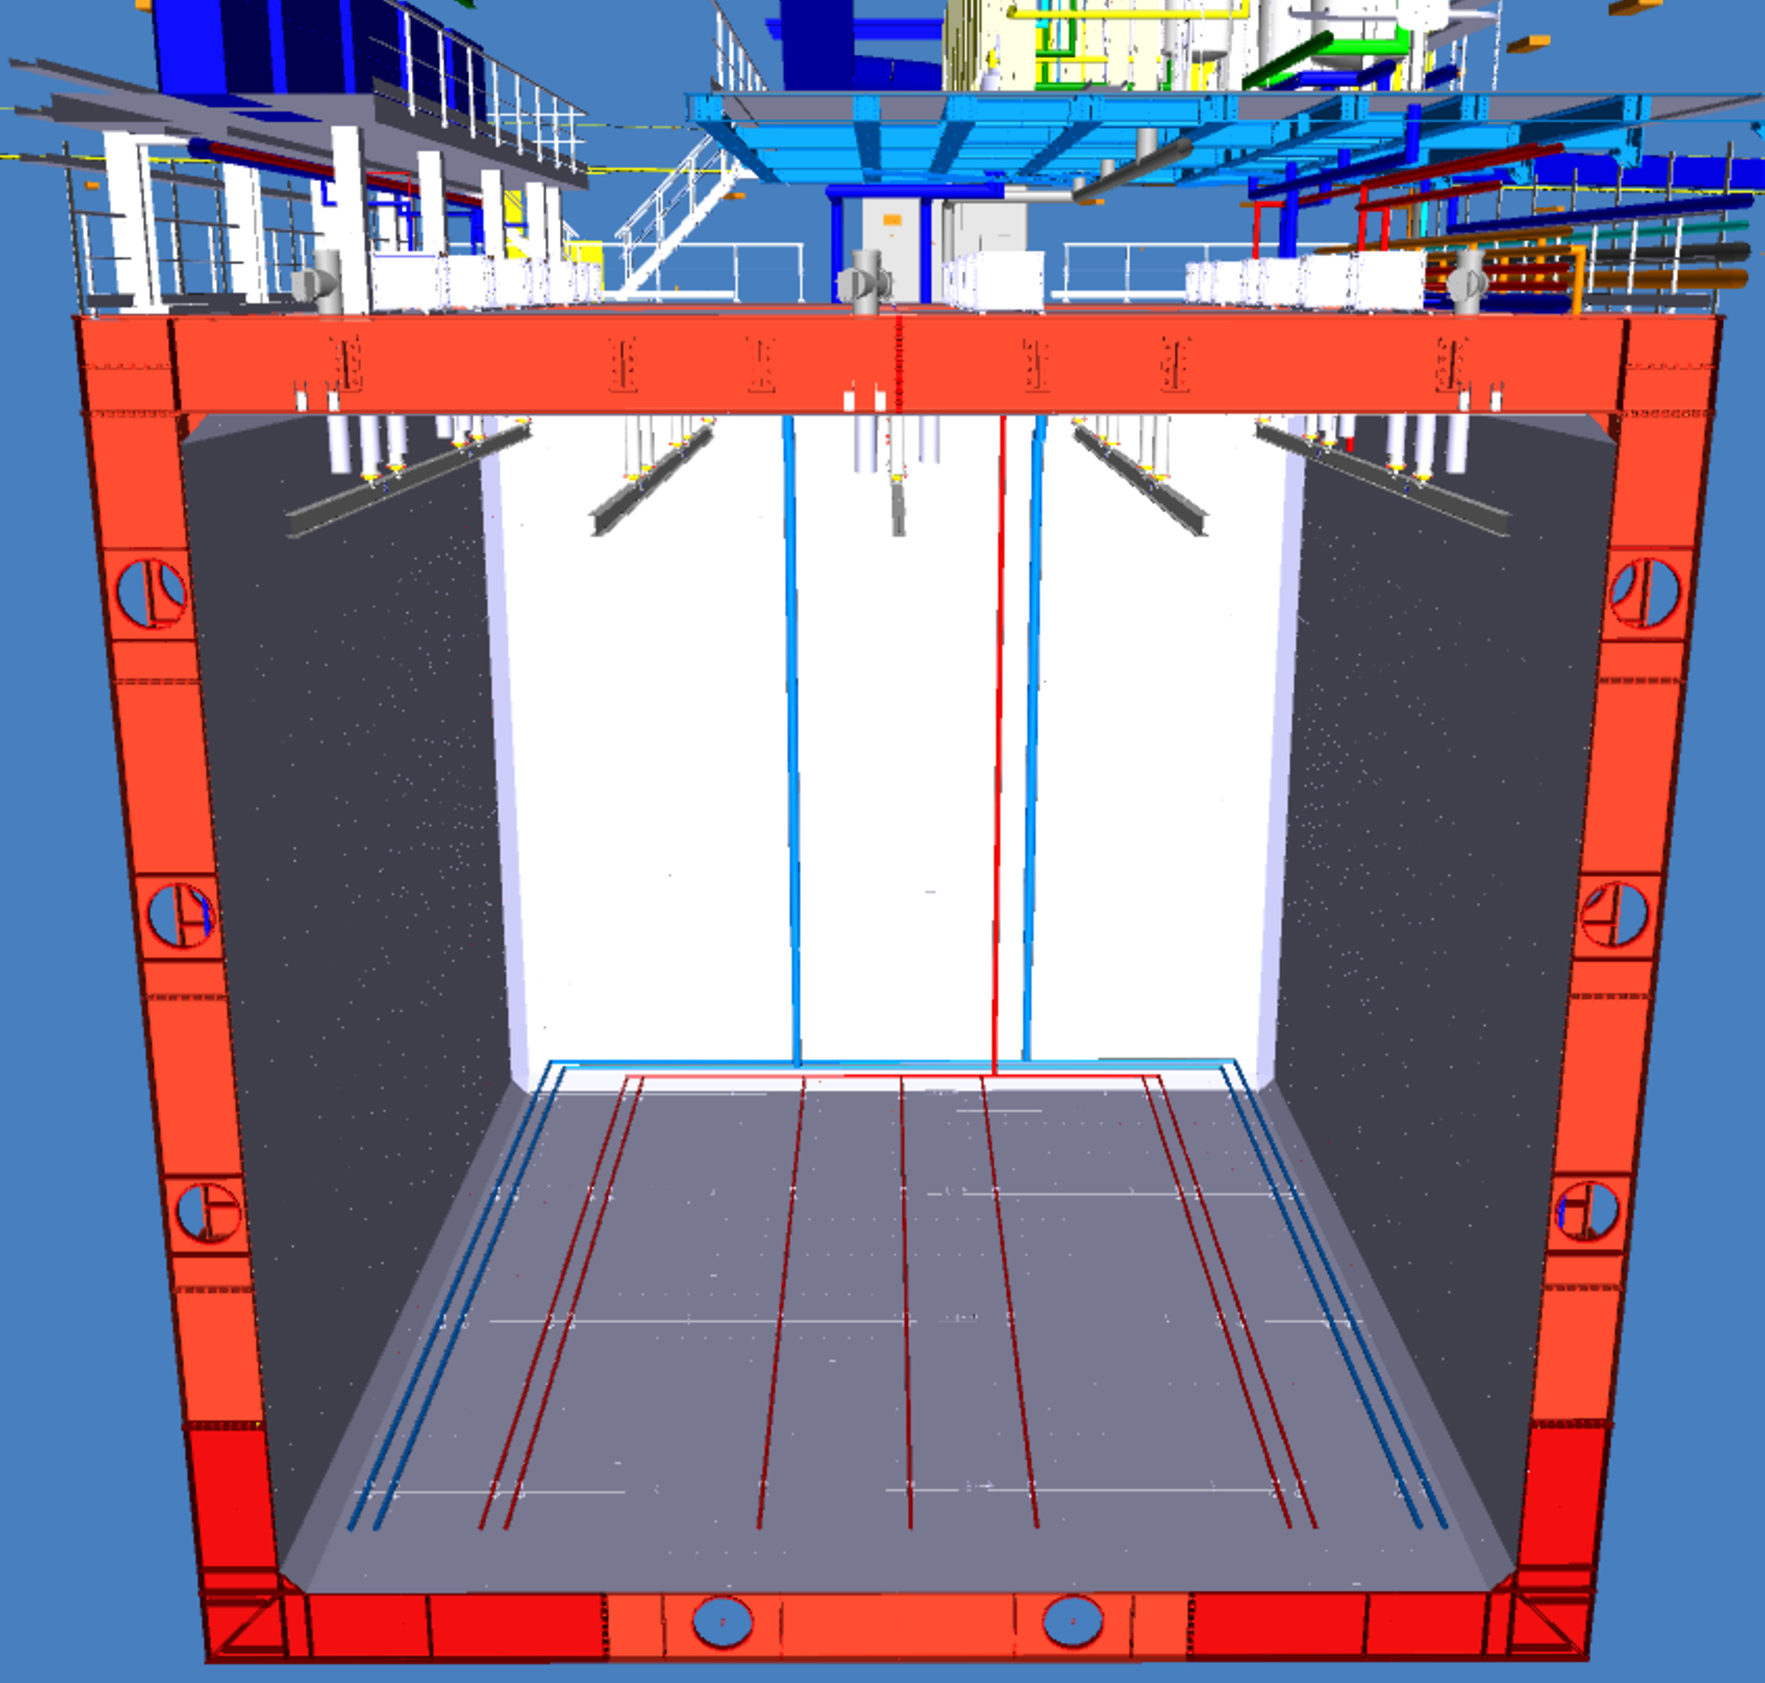
\includegraphics[width=.98\textwidth]{graphics/Internal-Piping-3D.pdf}
\end{dunefigure}

\begin{dunefigure}[Drawing of the cryogenic piping inside the cryostat ]{fig:internal-cryo-drawing}
  {Drawing of the internal cryogenics.}
%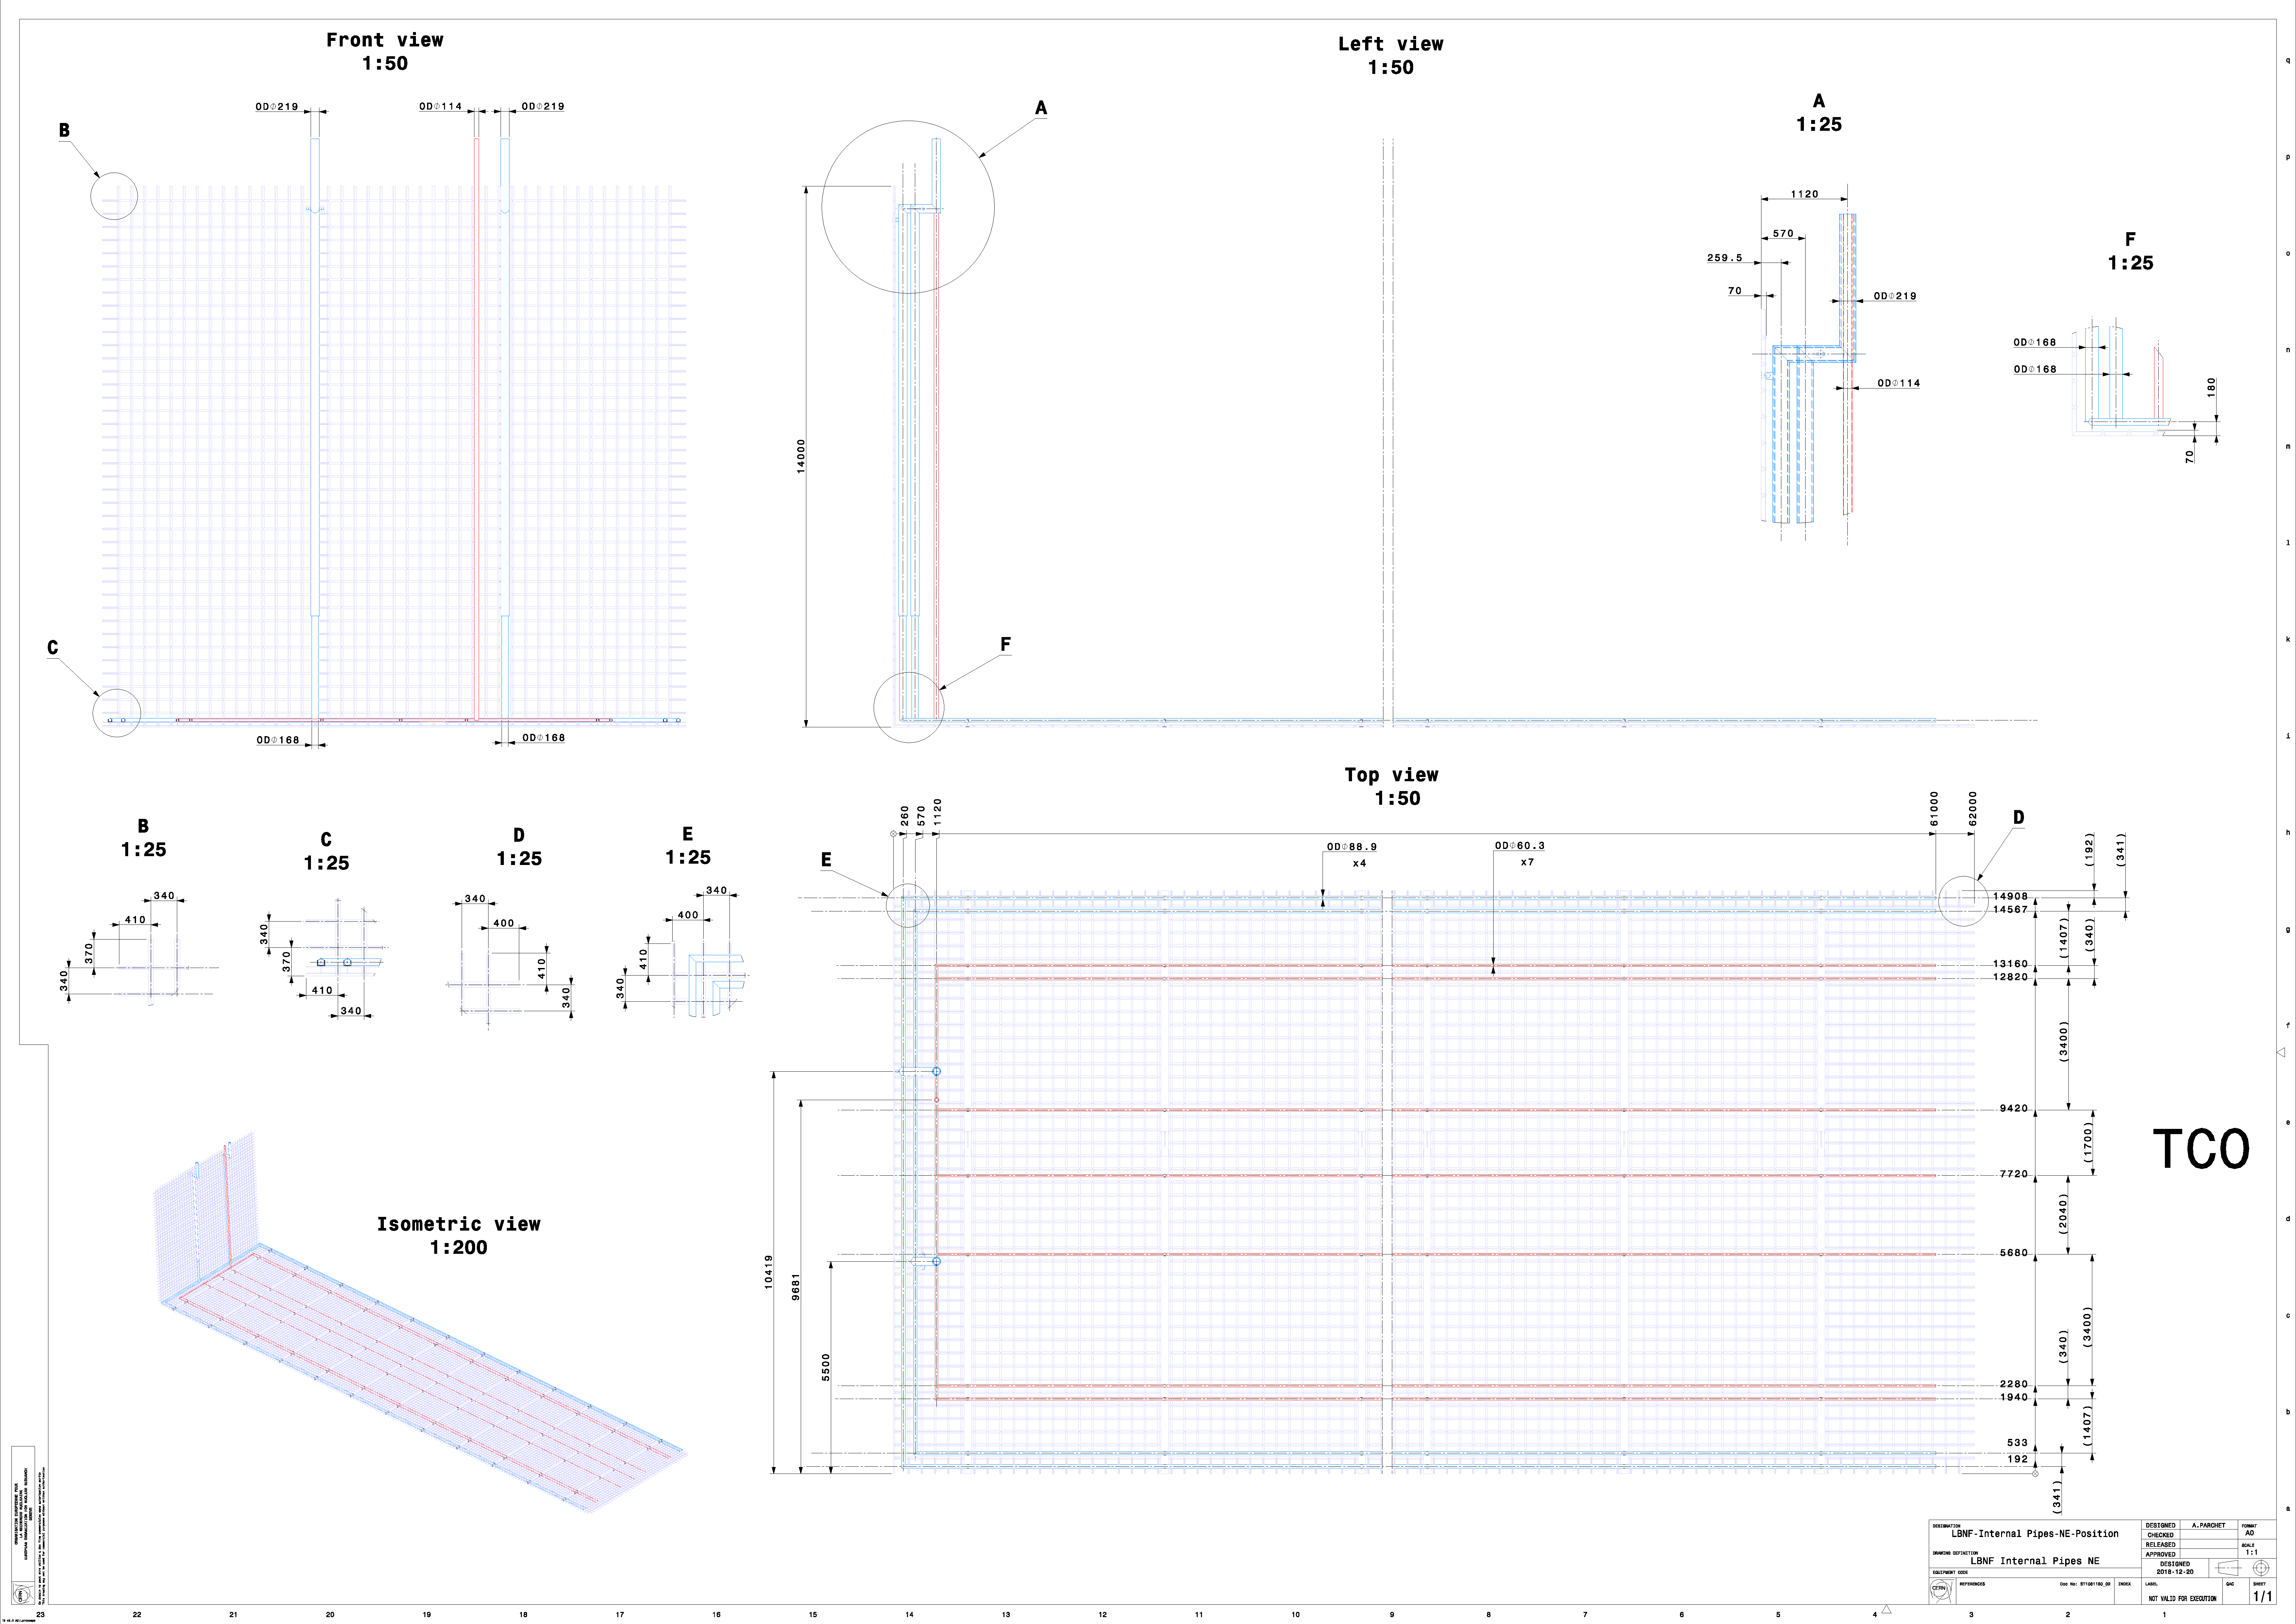
\includegraphics[angle=90,width=.98\textwidth]{graphics/Internal-pipes-HQ.pdf}
%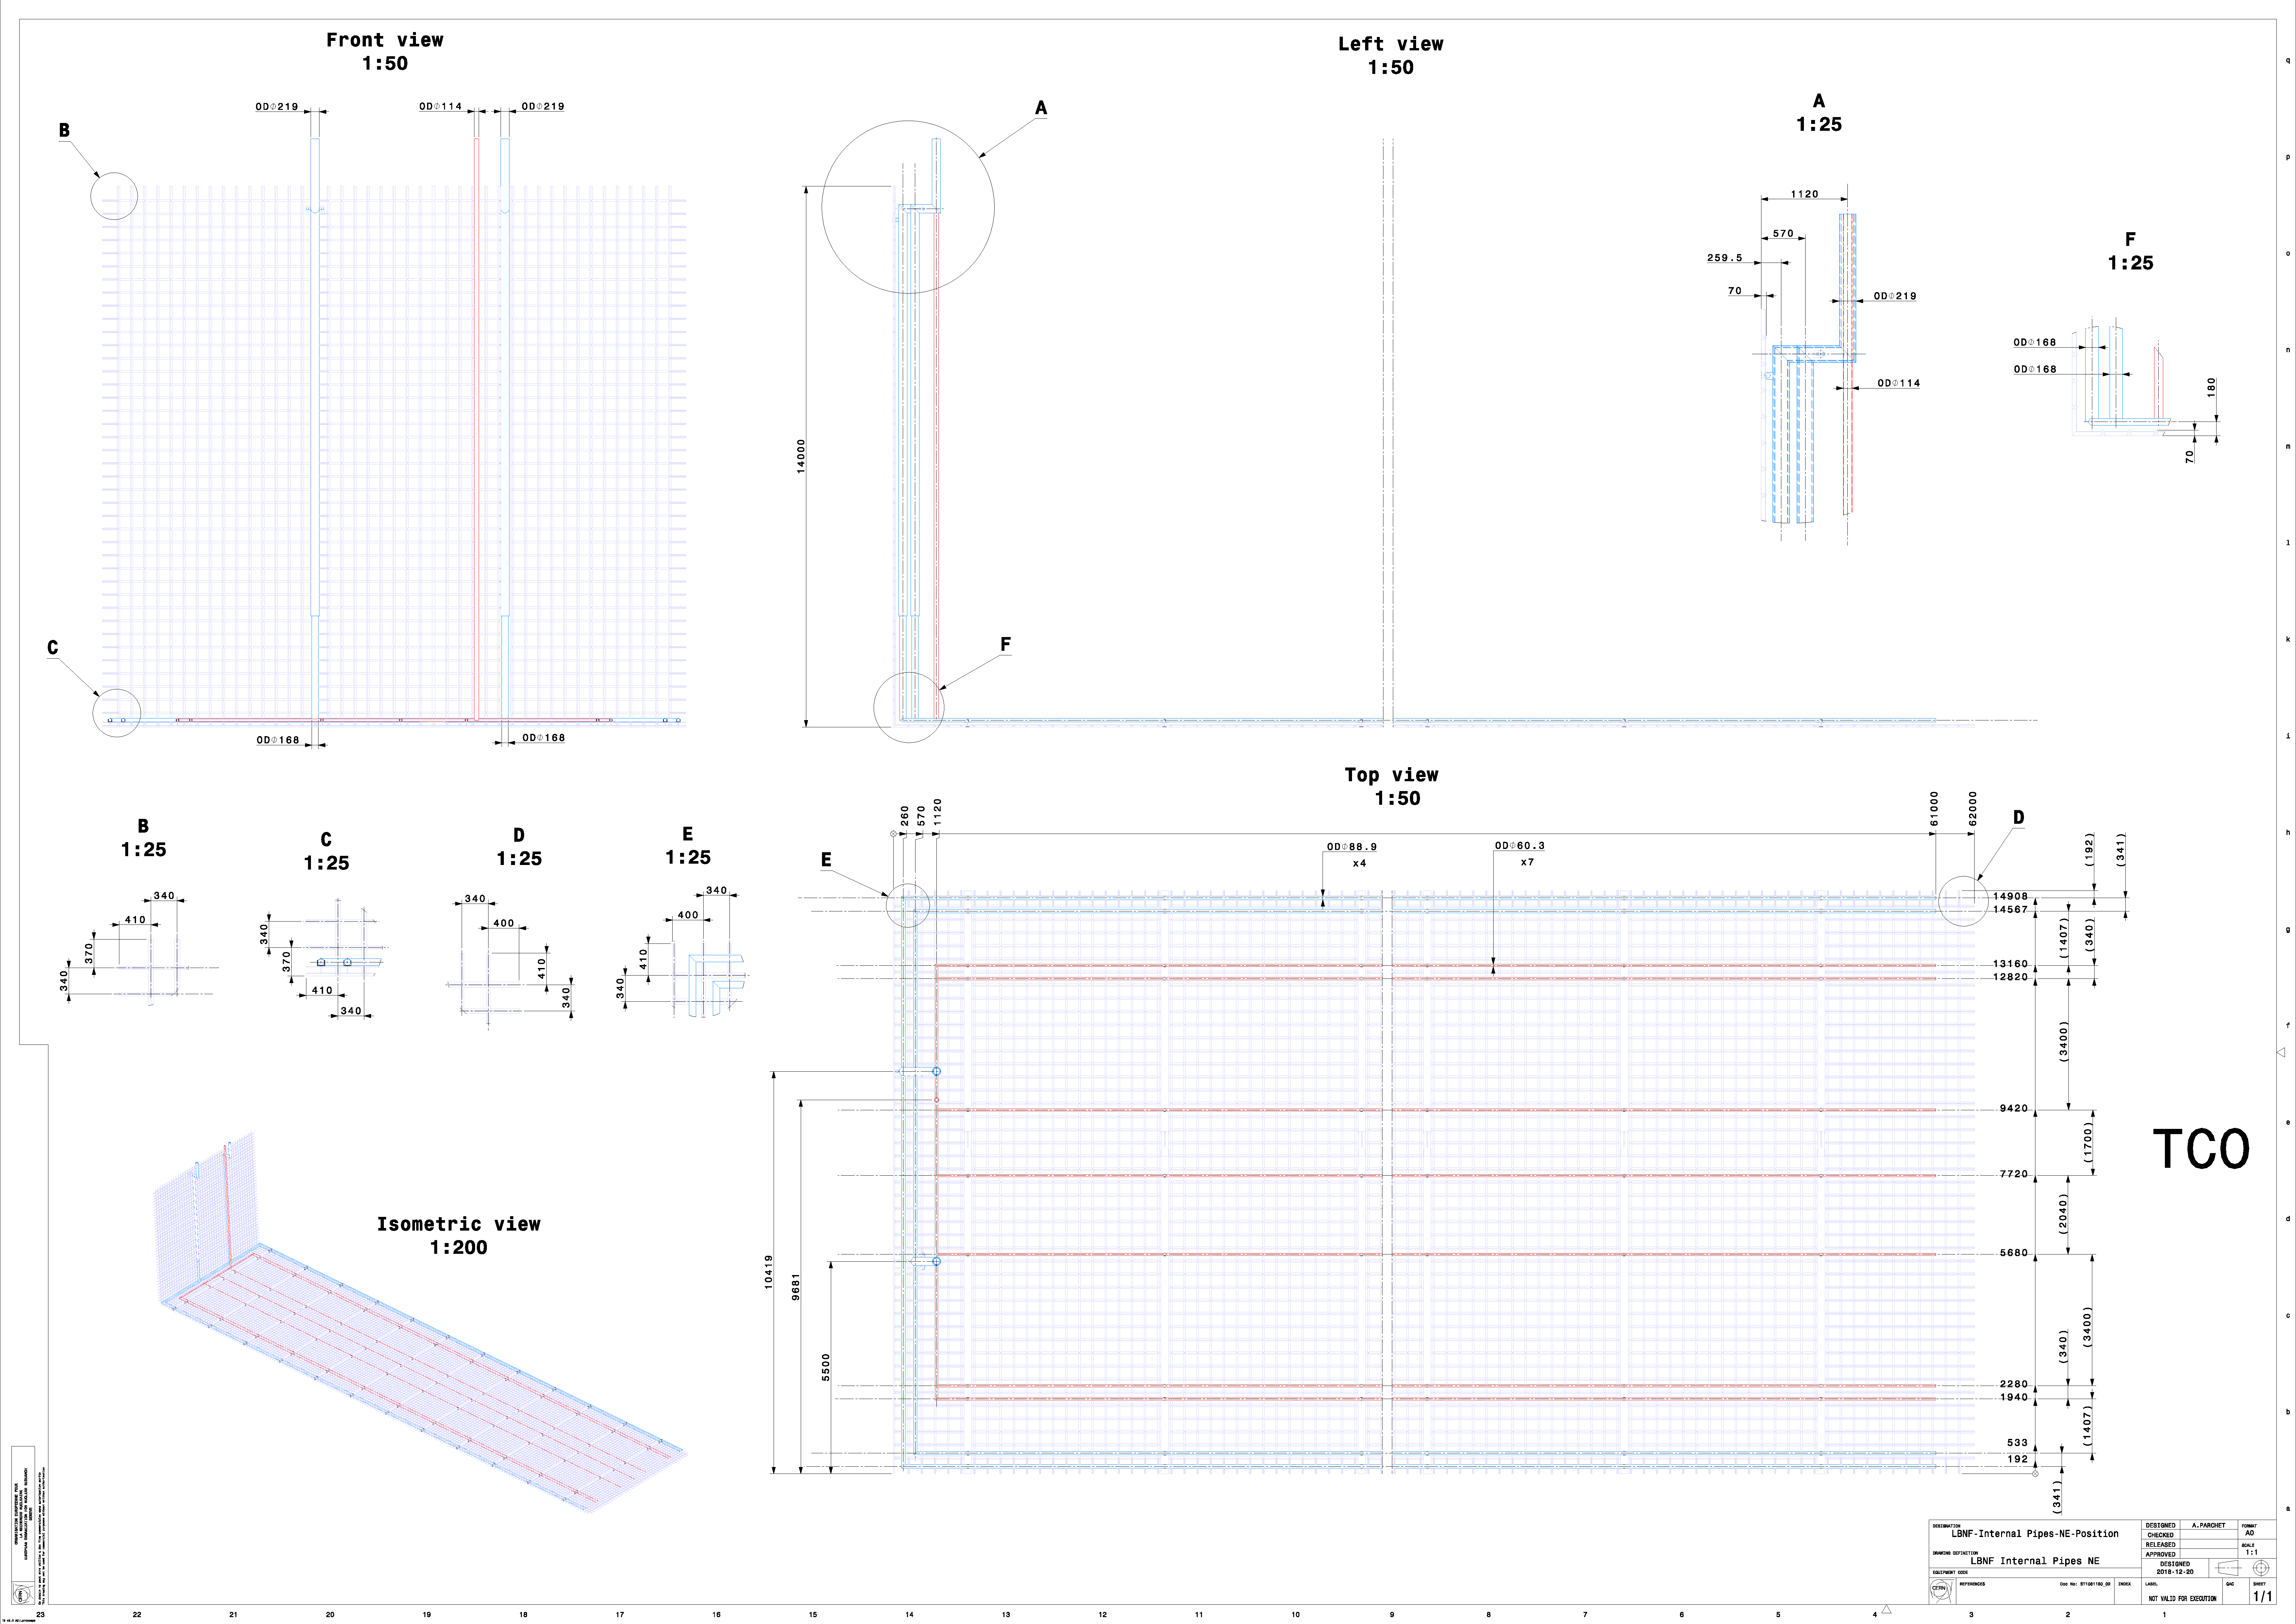
\includegraphics[angle=90,height=.98\textheight]{graphics/Internal-pipes-HQ.pdf}
\end{dunefigure}
\fixme{Please reduce size of Internal-pipes-HQ.pdf}
